%%%%%%%%%%%%%%%%%%%%%%%%%%%%%%%%%%%%%%%%%
% University/School Laboratory Report
% LaTeX Template
% Version 3.1 (25/3/14)
%
% This template has been downloaded from:
% http://www.LaTeXTemplates.com
%
% Original author:
% Linux and Unix Users Group at Virginia Tech Wiki 
% (https://vtluug.org/wiki/Example_LaTeX_chem_lab_report)
%
% License:
% CC BY-NC-SA 3.0 (http://creativecommons.org/licenses/by-nc-sa/3.0/)
%
%%%%%%%%%%%%%%%%%%%%%%%%%%%%%%%%%%%%%%%%%

%----------------------------------------------------------------------------------------
%	PACKAGES AND DOCUMENT CONFIGURATIONS
%----------------------------------------------------------------------------------------

\documentclass{article}

\usepackage[version=3]{mhchem} % Package for chemical equation typesetting
\usepackage{siunitx} % Provides the \SI{}{} and \si{} command for typesetting SI units
\usepackage{graphicx} % Required for the inclusion of images
\usepackage{natbib} % Required to change bibliography style to APA
\usepackage{amsmath} % Required for some math elements 
\usepackage[utf8]{inputenc}
\usepackage{tikz,pgfplots}
\usepackage[letterpaper, margin=0.2in]{geometry}
\usepackage{float}
\usepackage{enumitem}
\usepackage{fixltx2e}
\usepackage{gensymb}
\usepackage[hidelinks]{hyperref}
\usepackage[all]{hypcap}

\usepackage{xcolor}
\usepackage{listings}
\usepackage{color}

% Code color matlab definitions
\definecolor{codegreen}{rgb}{0,0.6,0}
\definecolor{codegray}{rgb}{0.5,0.5,0.5}
\definecolor{codepurple}{rgb}{0.58,0,0.82}
\definecolor{backcolour}{rgb}{0.95,0.95,0.92}
 
\lstdefinestyle{mystyle}{
    backgroundcolor=\color{backcolour},   
    commentstyle=\color{codegreen},
    keywordstyle=\color{magenta},
    numberstyle=\tiny\color{codegray},
    stringstyle=\color{codepurple},
    basicstyle=\footnotesize,
    breakatwhitespace=false,         
    breaklines=true,                 
    captionpos=b,                    
    keepspaces=true,                 
    numbers=left,                    
    numbersep=5pt,                  
    showspaces=false,                
    showstringspaces=false,
    showtabs=false,                  
    tabsize=2
}

\lstset{style=mystyle}

% Roman numerials
\pagenumbering{arabic}

\setlength\parindent{0pt} % Removes all indentation from paragraphs

%\renewcommand{\labelenumi}{\alph{enumi}.} % Make numbering in the enumerate environment by letter rather than number (e.g. section 6)

%\usepackage{times} % Uncomment to use the Times New Roman font

% for some tables
\newcommand{\specialcell}[2][c]{%
  \begin{tabular}[#1]{@{}c@{}}#2\end{tabular}}
  
\providecommand{\e}[1]{\ensuremath{\times 10^{#1}}}
%----------------------------------------------------------------------------------------
%	DOCUMENT INFORMATION
%----------------------------------------------------------------------------------------

%\title{Determination of the Atomic \\ Weight of Magnesium \\ CHEM 101} % Title

%\author{John \textsc{Smith}} % Author name

%\date{\today} % Date for the report
\title{KeySight u2701A Modular Scope tests with Matlab}
\author{Levon Dovlatyan}
\date{\today}
\begin{document}

%\maketitle % Insert the title, author and date

% If you wish to include an abstract, uncomment the lines below
% \begin{abstract}
% Abstract text
% \end{abstract}

%----------------------------------------------------------------------------------------
%	SECTION 1
%----------------------------------------------------------------------------------------

\begin{figure}[H]
\centering
\begin{tikzpicture}
\node at (-5,0) {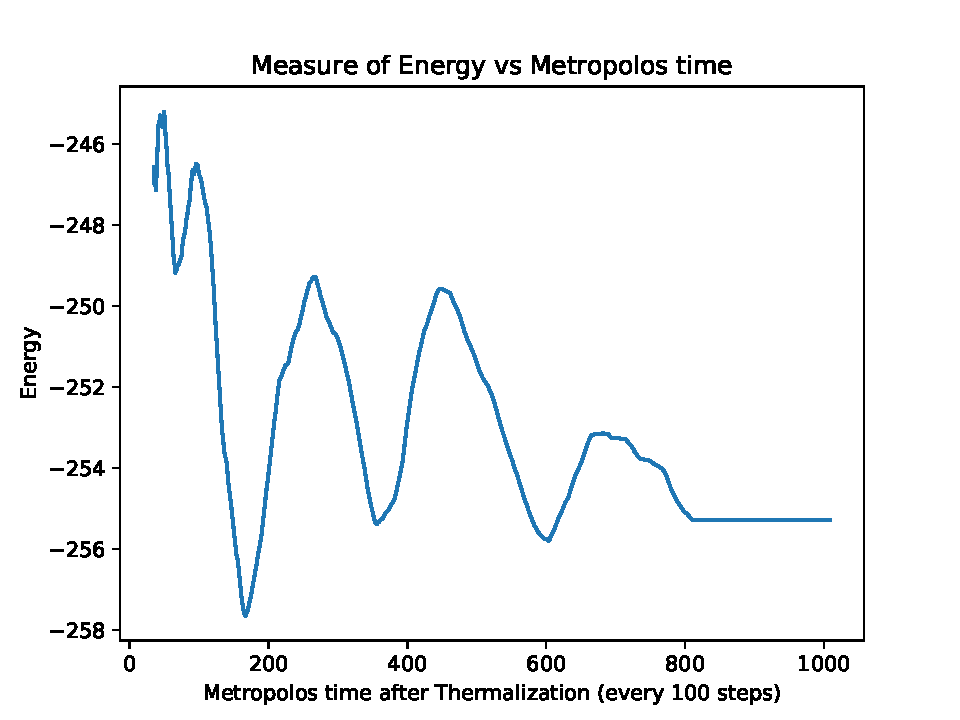
\includegraphics[width=300pt]{p2_Energy.pdf}};
\node at (5,0) {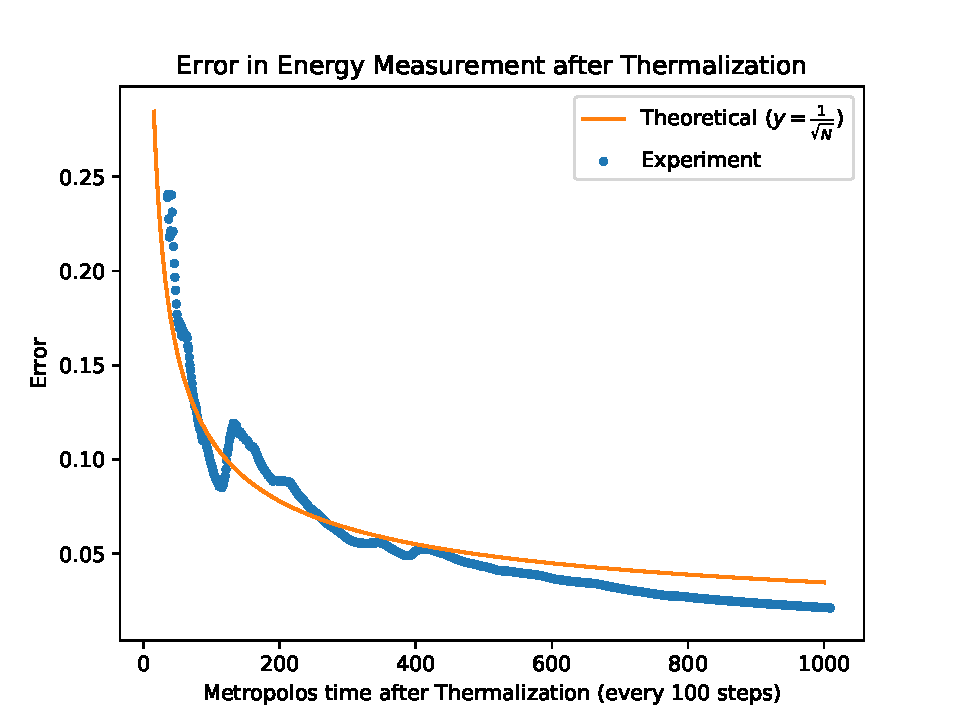
\includegraphics[width=300pt]{p2_error.pdf}};
\end{tikzpicture}
\end{figure}

\begin{figure}[H]
\centering
\begin{tikzpicture}
\node at (-5,0) {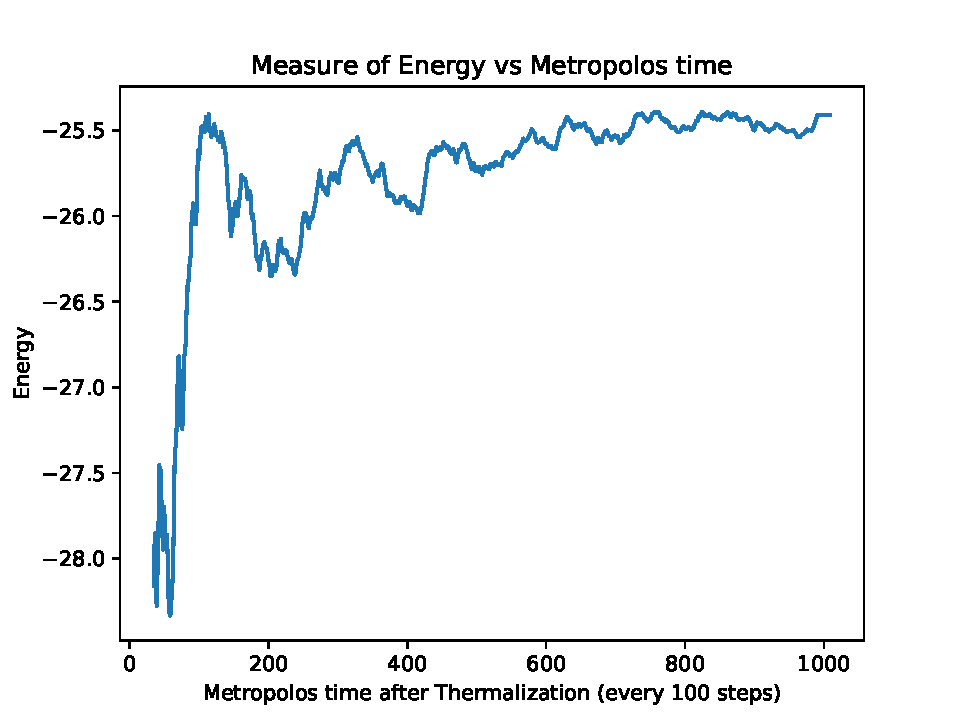
\includegraphics[width=300pt]{p3_100_Energy.pdf}};
\node at (5,0) {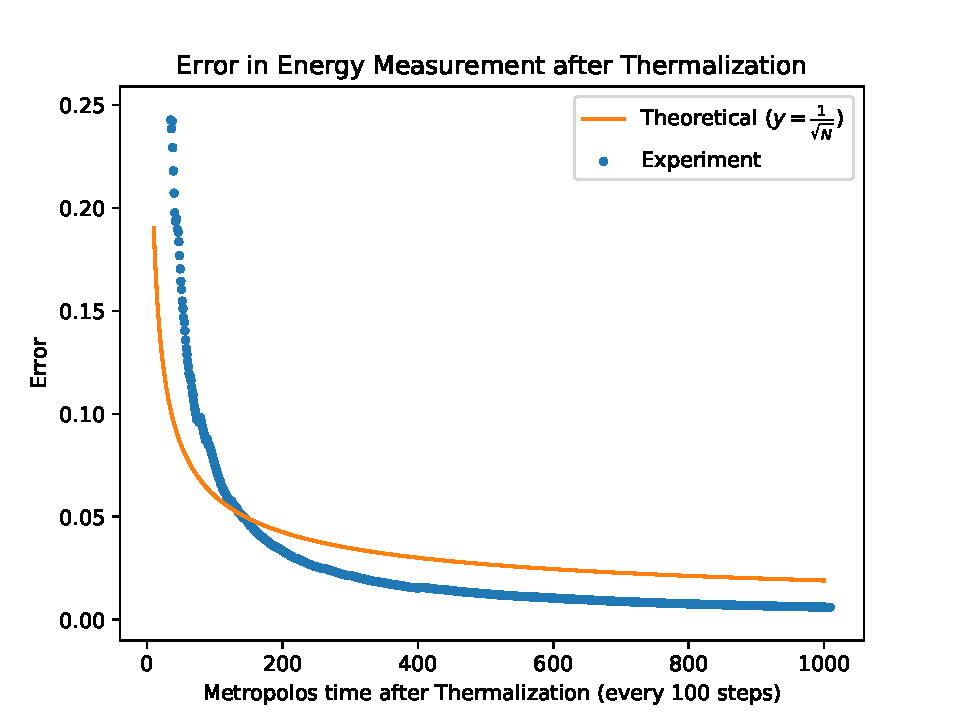
\includegraphics[width=300pt]{p3_100_Error.pdf}};
\end{tikzpicture}
\end{figure}

\begin{figure}[H]
\centering
\begin{tikzpicture}
\node at (-5,0) {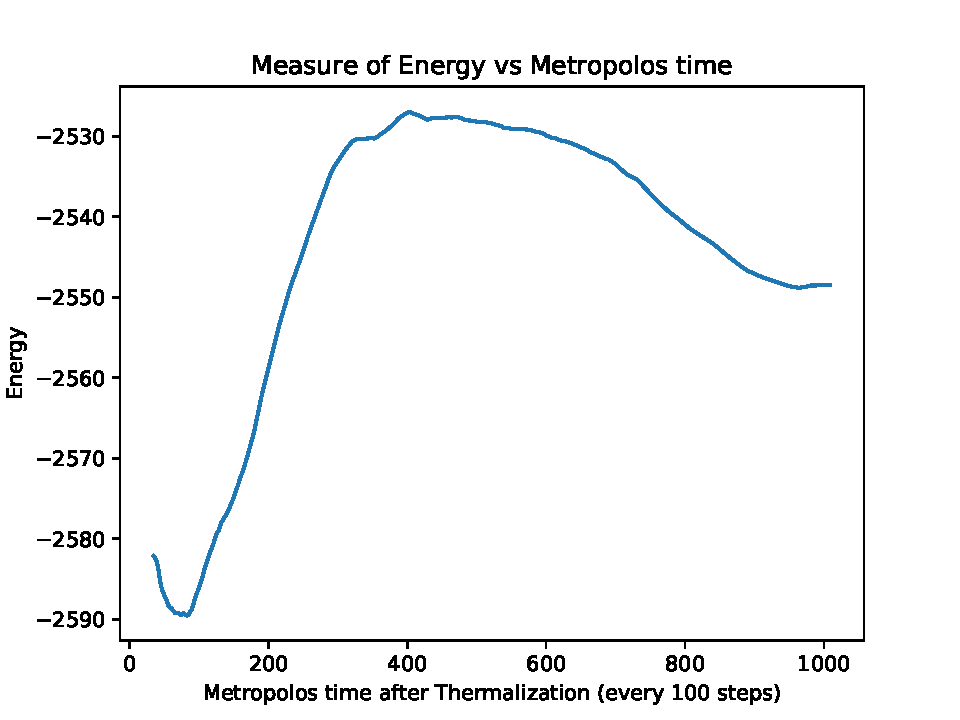
\includegraphics[width=300pt]{p3_10000_Energy.pdf}};
\node at (5,0) {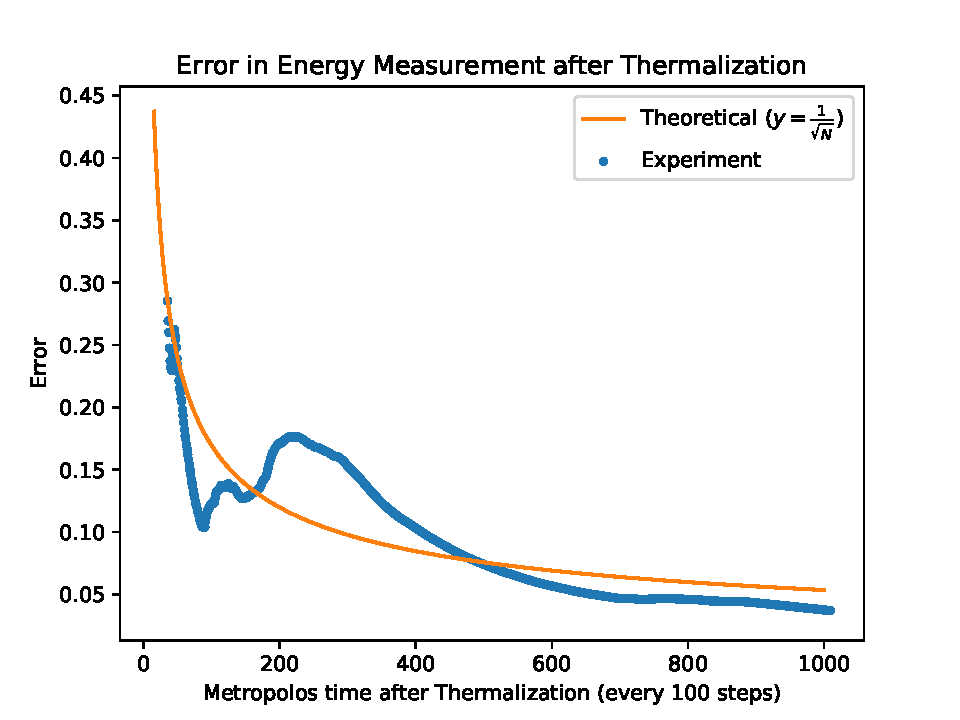
\includegraphics[width=300pt]{p3_10000_Error.pdf}};
\end{tikzpicture}
\end{figure}

\begin{figure}[H]
\centering
\begin{tikzpicture}
\node at (-5,0) {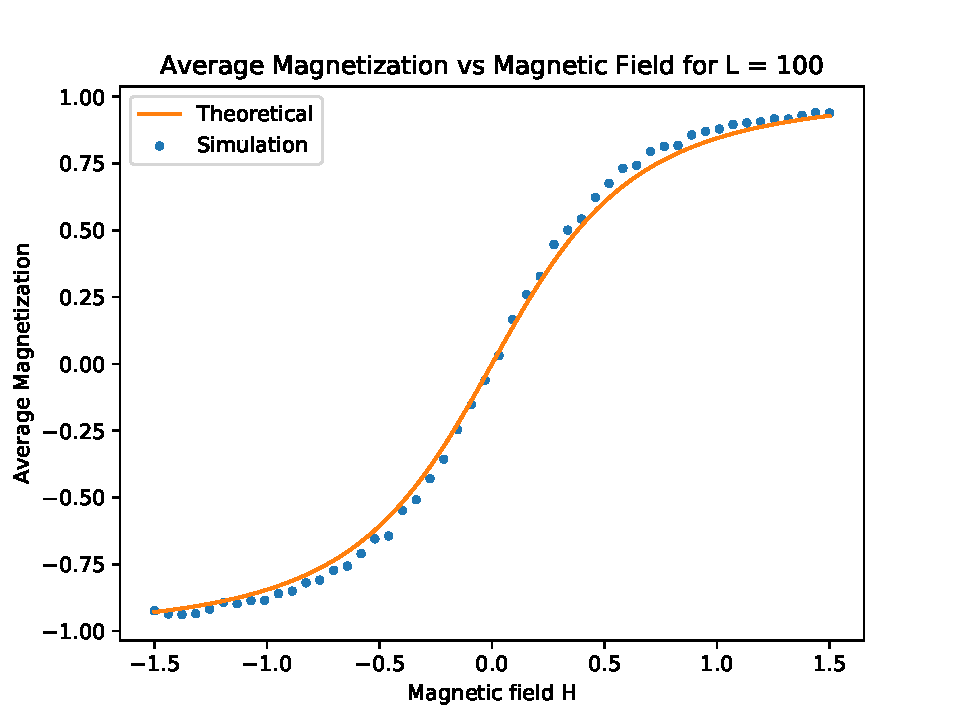
\includegraphics[width=300pt]{p5_100.pdf}};
\node at (5,0) {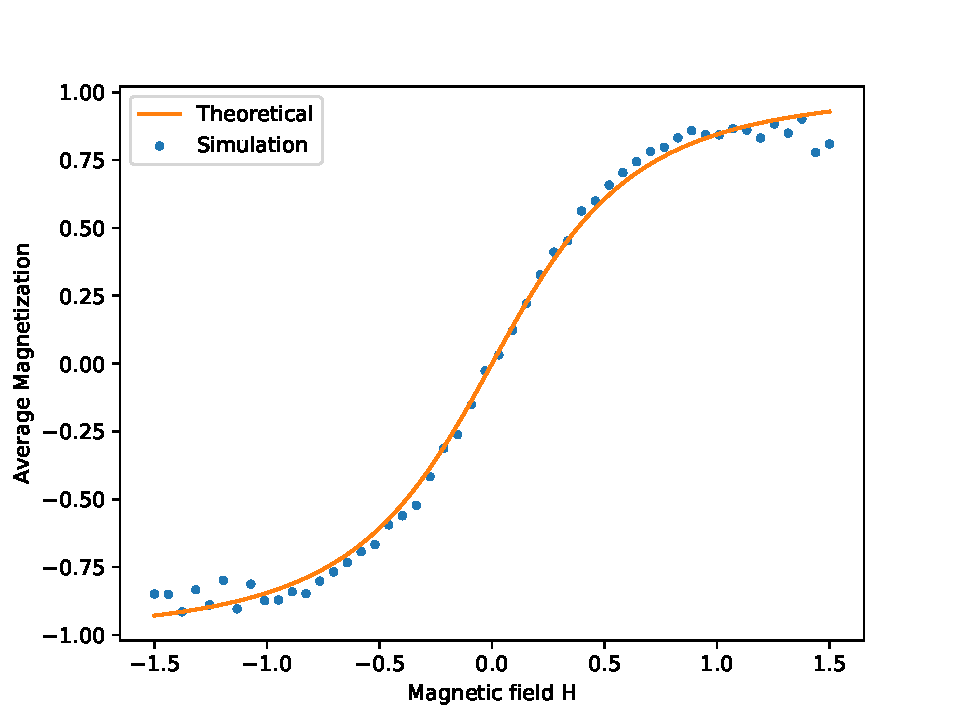
\includegraphics[width=300pt]{p5.pdf}};
\end{tikzpicture}
\end{figure}

\begin{figure}[H]
\centering
\begin{tikzpicture}
\node at (-5,0) {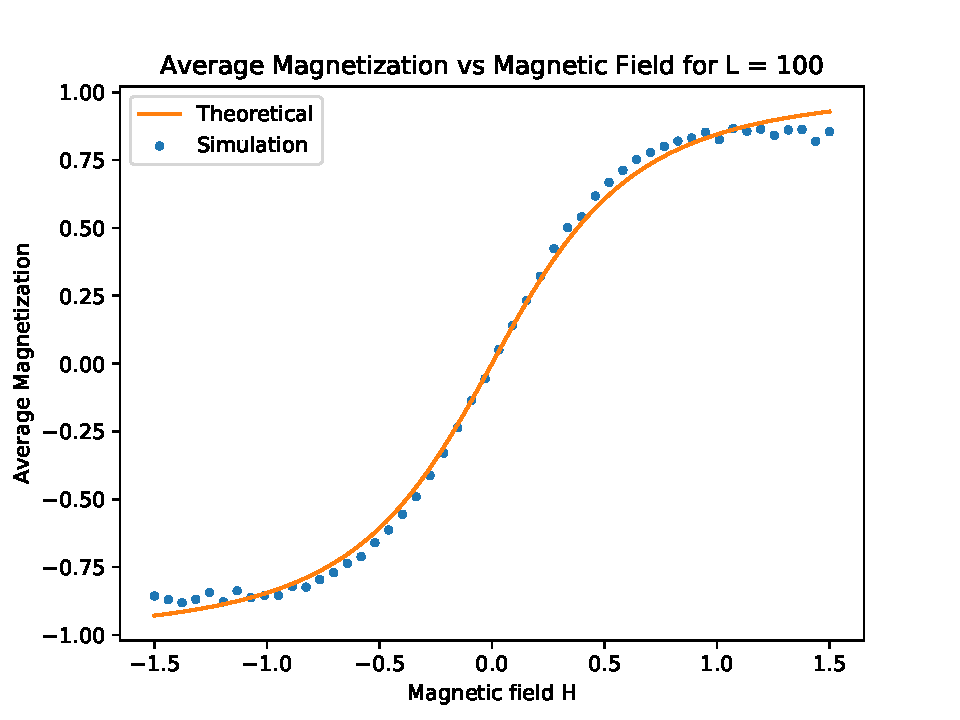
\includegraphics[width=300pt]{p5_10000.pdf}};
\node at (5,0) {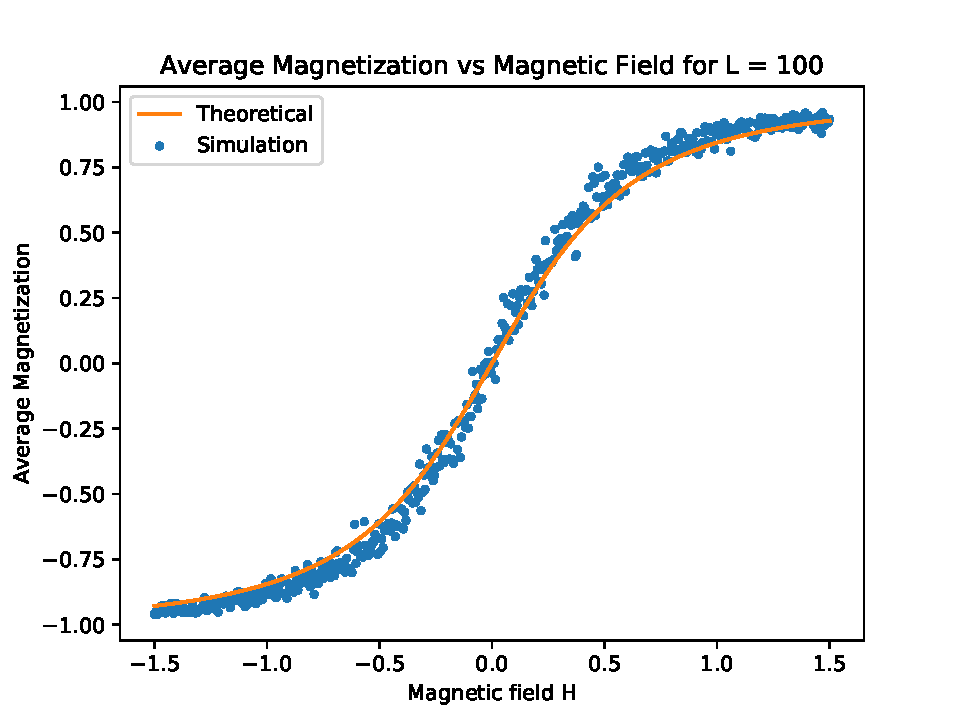
\includegraphics[width=300pt]{p5_100_500pts.pdf}};
\end{tikzpicture}
\end{figure}

\begin{figure}[H]
\centering
\begin{tikzpicture}
\node at (-5,0) {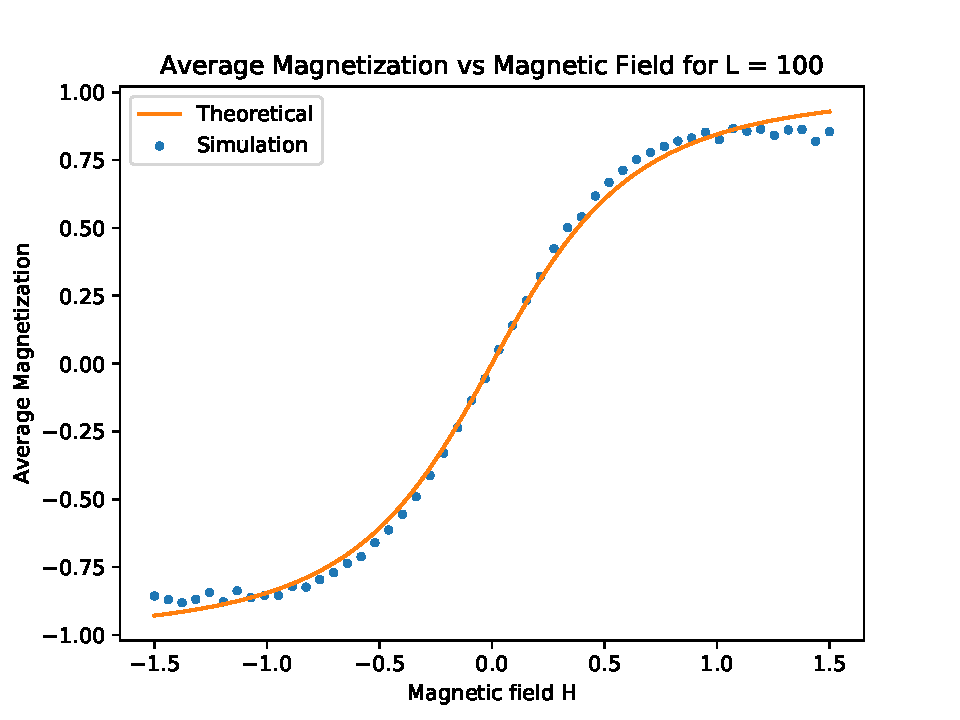
\includegraphics[width=300pt]{p5_10000.pdf}};
\node at (5,0) {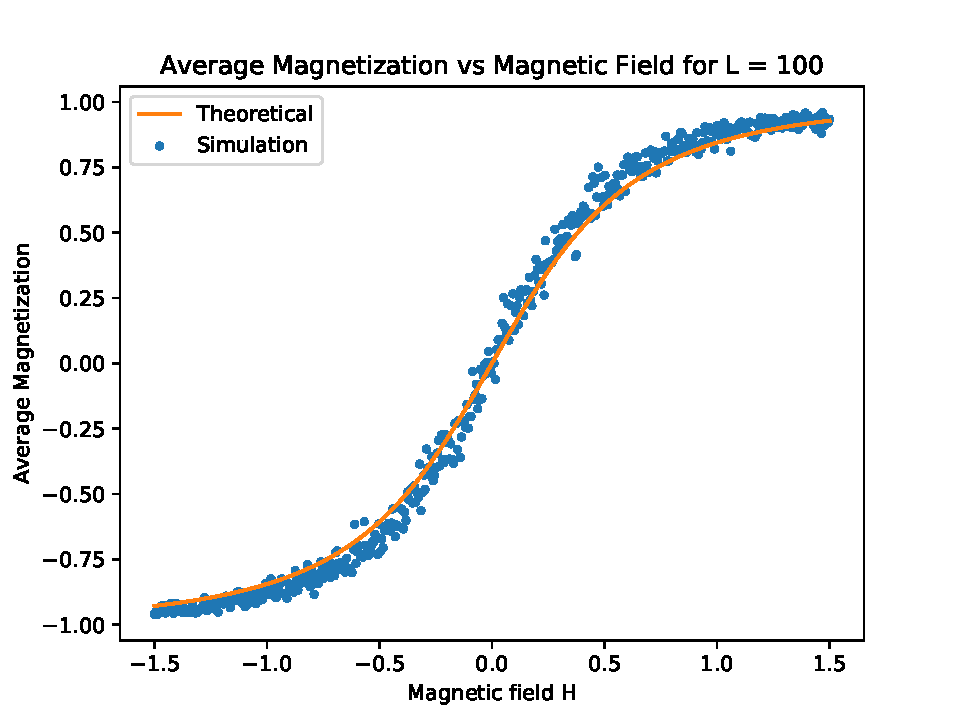
\includegraphics[width=300pt]{p5_100_500pts.pdf}};
\end{tikzpicture}
\end{figure}

\begin{figure}[H]
\centering
\begin{tikzpicture}
\node at (0,0) {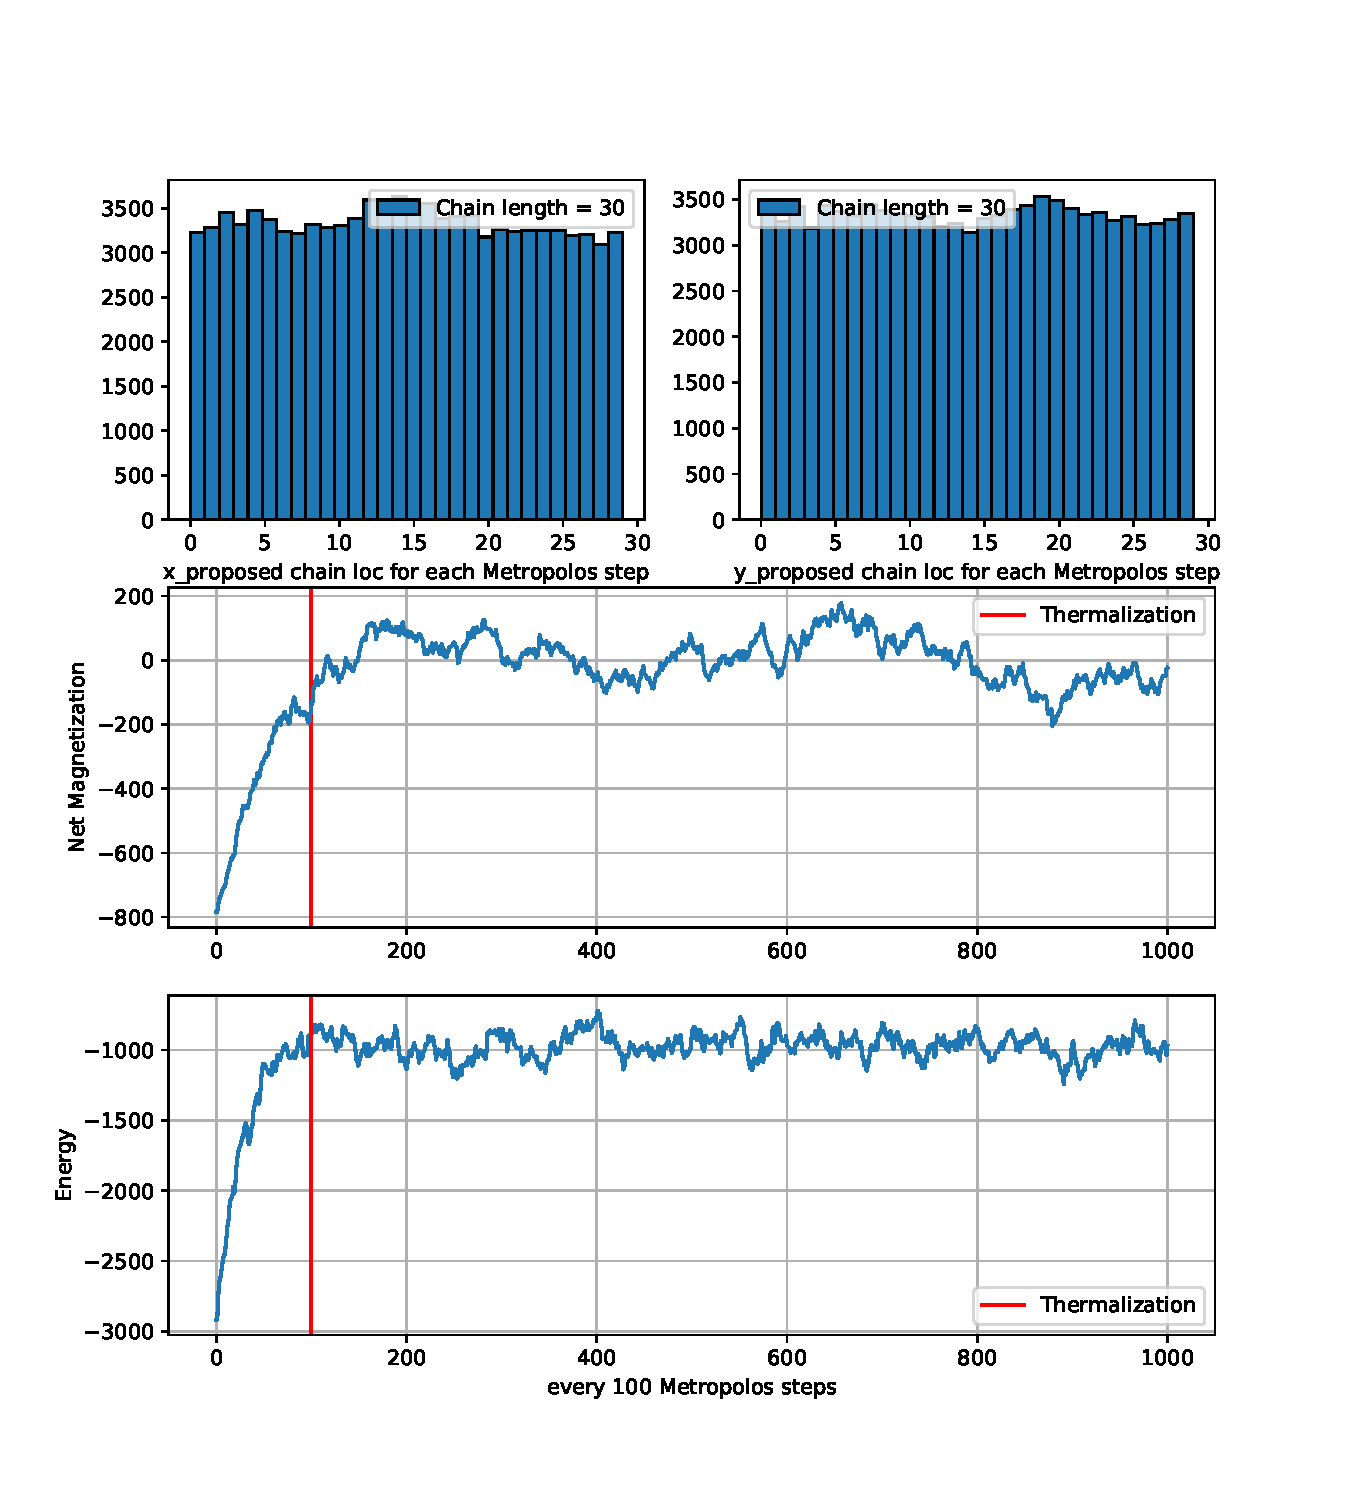
\includegraphics[width=600pt]{2d_p2.pdf}};
\end{tikzpicture}
\end{figure}

\begin{figure}[H]
\centering
\begin{tikzpicture}
\node at (0,0) {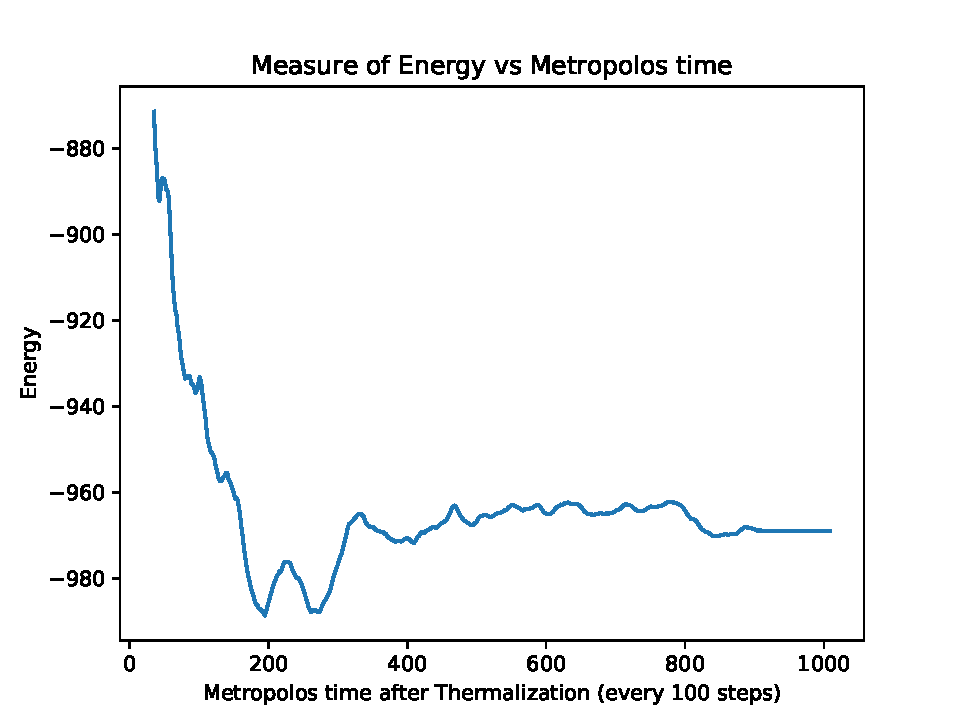
\includegraphics[width=300pt]{2d_p3_energy_n30.pdf}};
\end{tikzpicture}
\end{figure}

\begin{figure}[H]
\centering
\begin{tikzpicture}
\node at (0,0) {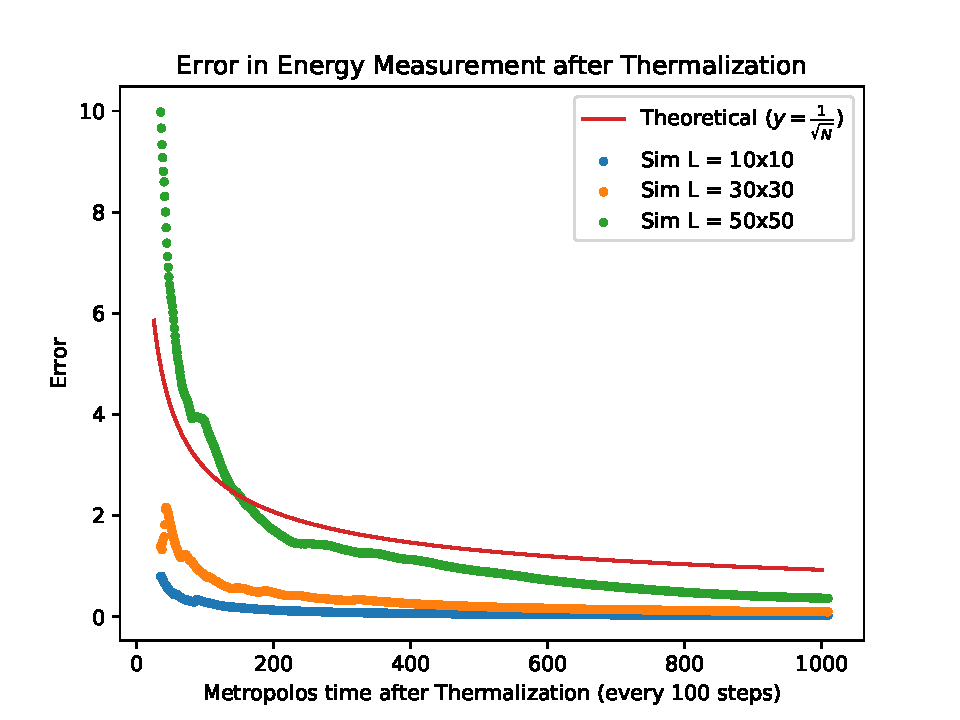
\includegraphics[width=300pt]{2d_p3_error_scale.pdf}};
\end{tikzpicture}
\end{figure}

\begin{figure}[H]
\centering
\begin{tikzpicture}
\node at (0,0) {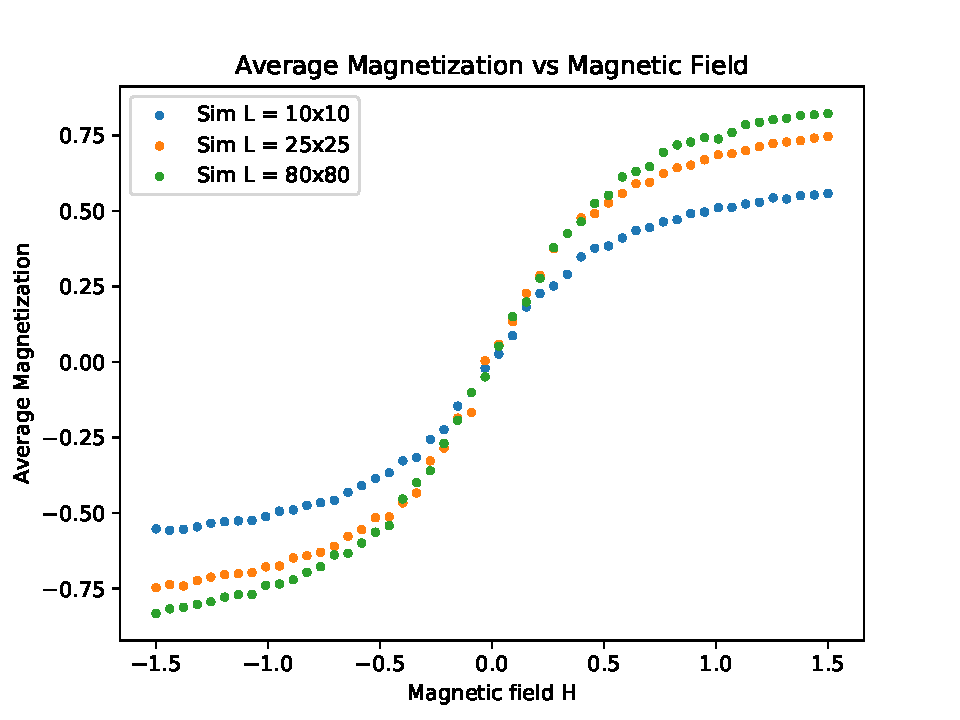
\includegraphics[width=300pt]{2d_p5.pdf}};
\end{tikzpicture}
\end{figure}








%\textcolor{white}{l} \\*[2cm]


% Nothing right now

%----------------------------------------------------------------------------------------
%	BIBLIOGRAPHY
%----------------------------------------------------------------------------------------

\bibliographystyle{apalike}

\bibliography{sample}

%----------------------------------------------------------------------------------------


\end{document}
